\documentclass{standalone}
\usepackage{pgfplots}
\pgfplotsset{compat=1.13}

\begin{document}

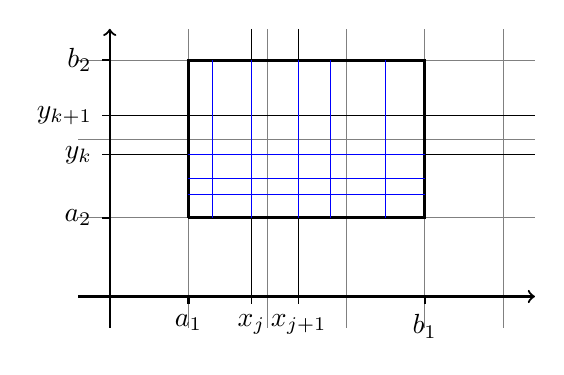
\begin{tikzpicture}
    \draw[step=1cm,gray,very thin] (-0.4,-0.4) grid (5.4,3.4);
    \draw[thick,->] (-0.4,0) -- (5.4,0);
    \draw[thick,->] (0,-0.4) -- (0,3.4);
    \draw[very thick] (1,1) -- (4,1) -- (4,3) -- (1,3) -- (1,1);
    \draw[thick] (1,0) -- (1,-.1) node[below] {\(a_1\)};
    \draw[thick] (4,0) -- (4,-.1) node[below] {\(b_1\)};
    \draw[thick] (0,1) -- (-.1,1) node[left] {\(a_2\)};
    \draw[thick] (0,3) -- (-.1,3) node[left] {\(b_2\)};
    \draw[] (5.4,1.8) -- (-.1,1.8) node[left] {\(y_{k}\)};
    \draw[] (5.4,2.3) -- (-.1,2.3) node[left] {\(y_{k+1}\)};
    \draw[blue]
    (1,1.3) -- (4,1.3)
    (1,1.5) -- (4,1.5)
    (1,1.8) -- (4,1.8);
    (1,2.3) -- (4,2.3)
    \draw[] (1.8,3.4) -- (1.8,-.1) node[below] {\(x_j\)};
    \draw[] (2.4,3.4) -- (2.4,-.1) node[below] {\(x_{j+1}\)};
    \draw[blue]
    (1.3,1) -- (1.3,3)
    (1.8,1) -- (1.8,3)
    (2.4,1) -- (2.4,3)
    (2.8,1) -- (2.8,3)
    (3.5,1) -- (3.5,3);
\end{tikzpicture}

\end{document}